\documentclass[aspectratio=169,11pt]{beamer}

\usepackage[T1]{fontenc}
\usepackage[utf8]{inputenc}
\usepackage[english]{babel}
\usepackage{booktabs}
\usepackage{graphicx}
\usepackage{tikz}
\usetikzlibrary{arrows.meta,positioning,fit,backgrounds}

% ---------------------------------------------------------------------------
% Clean, theme-light setup: no navigation clutter, one accent colour.
% ---------------------------------------------------------------------------
\usetheme{default}
\usecolortheme{default}

% Notes build: slides-notes.tex sets \SHOWNOTES and \input's this file, so the
% spoken script lives in exactly one place -- the \note{} blocks below.
\usepackage{pgfpages}
\ifdefined\SHOWNOTES\setbeameroption{show notes}\fi

\definecolor{ctublue}{RGB}{0,101,189}
\definecolor{accent}{RGB}{200,16,46}
\setbeamercolor{structure}{fg=ctublue}
\setbeamercolor{title}{fg=ctublue}
\setbeamercolor{frametitle}{fg=ctublue}
\setbeamerfont{frametitle}{size=\large,series=\bfseries}
\setbeamertemplate{navigation symbols}{}
\setbeamertemplate{itemize items}[circle]
\setbeamertemplate{footline}{%
  \hfill\usebeamerfont{footline}\color{gray!70}%
  \small\insertframenumber\,/\,\inserttotalframenumber\hspace*{2ex}\vspace*{1ex}%
}

\newcommand{\gtcc}[1]{\textbf{\color{accent}#1}}

% ---------------------------------------------------------------------------

\title[Acoustic Detection of Impulsive Sounds]{Acoustic-Based Detection, Classification,\\and Localization of Impulsive Sounds}
\author{Jakub Svatoš \and \underline{Martin Maxa}}
\institute{Czech Technical University in Prague\\Faculty of Electrical Engineering, Department of Measurement}
% TODO: replace the placeholder with the confirmed conference name and city.
\date{{\color{accent}$\langle$CONFERENCE NAME --- TO BE CONFIRMED$\rangle$}\\[3pt]
      September 16, 2026}

\begin{document}

\begin{frame}[plain]
  \titlepage
  \note{%
    \textbf{[0:00--0:30]}\par\medskip
    Good morning. // My name is Martin Maxa, from the Czech Technical University
    in Prague, Department of Measurement. // I am presenting joint work with
    Doctor Jakub Svatoš. //\par\medskip
    Our topic is acoustic detection, classification and localization of impulsive
    sounds --- in practice, gunshots. // I will show you how we detect them, how we
    tell them apart, and how we find where they came from. //\par\medskip
    \textit{(// = pause. [CLICK] = advance the slide.)}
  }
\end{frame}

% ===========================================================================
\section{Motivation}

\begin{frame}{Why acoustic surveillance}
  \begin{itemize}
    \item Shootings in public spaces are more frequent; global gun ownership is rising.
    \item Growing demand for autonomous security in communal areas --- campuses,
          hospitals, parks, government facilities.
    \item Cameras, drones and security personnel give \emph{some} protection, but
          fall short in high-risk situations with an active shooter.
  \end{itemize}
  \vfill
  \begin{block}{What an acoustic system adds}
    Identifies gunfire, pinpoints its source, and tracks an ongoing threat ---
    faster detection and shorter response times for security forces.
  \end{block}
  \note{%
    \textbf{[0:30--1:15]}\par\medskip
    Shootings in public spaces are becoming more frequent, and gun ownership is
    rising worldwide. // At the same time there is growing demand for autonomous
    security in places where people gather --- campuses, hospitals, parks,
    government buildings. //\par\medskip
    Cameras, drones and security staff already give some protection. But in a
    high-risk situation, with an active shooter, they fall short. // A camera has to
    be pointed the right way. A guard has to be in the right place. //\par\medskip
    Sound does not care about line of sight. An acoustic system hears the shot and
    tells you where it came from. //
  }
\end{frame}

% ===========================================================================
\section{Signal}

\begin{frame}{The acoustic signature of a gunshot}
  \begin{columns}[T,onlytextwidth]
    \begin{column}{0.62\textwidth}
      \vspace{-2mm}
      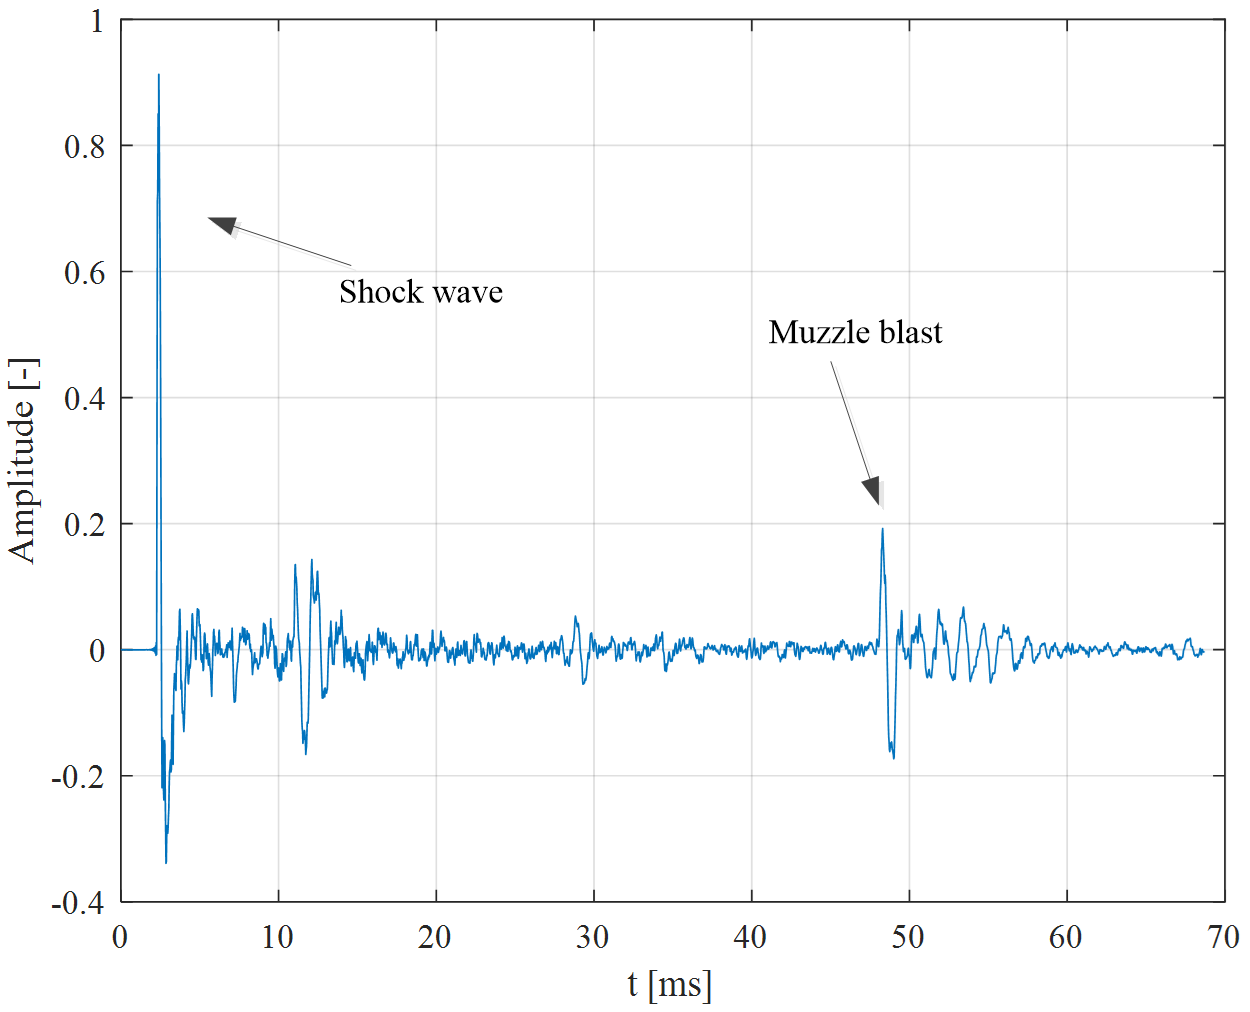
\includegraphics[width=\textwidth]{figs/gunshot_char.png}
    \end{column}
    \begin{column}{0.36\textwidth}
      \vspace{4mm}
      \begin{itemize}\small
        \item \textbf{Shock wave} (``N-wave'') --- arrives \emph{first}; exists only
              when the bullet is supersonic ($v > c$).
        \pause
        \item \textbf{Muzzle blast} --- gases leaving the barrel, 1--3\,ms; travels
              at the speed of sound, so it arrives $\approx$45\,ms later.
        \item Everything between and after: \gtcc{reflections}.
      \end{itemize}
    \end{column}
  \end{columns}
  \note<2>{%
    \textbf{[1:15--2:30]}\par\medskip
    So what does a gunshot look like to a microphone? // This is a real recording.
    Two components define the pattern --- and notice that they do not arrive together.
    //\par\medskip
    The first spike, at about two and a half milliseconds, is the shock wave. It
    exists only when the bullet travels faster than sound. The bullet drags a cone of
    compressed air behind it, and that cone sweeps across the microphone. That is the
    characteristic N shape. //\par\medskip
    \textbf{[CLICK]}\par\medskip
    The second spike, forty-five milliseconds later, is the muzzle blast --- the
    explosive gases leaving the barrel. It leaves the weapon at the instant of firing,
    but it only travels at the speed of sound, so it arrives late. It lasts one to
    three milliseconds. //\par\medskip
    Now look at everything in between and after. That is no longer the gunshot ---
    those are reflections from the surroundings. Remember that; it comes back at the
    end of the talk. //
  }
\end{frame}

\begin{frame}{Why naive processing is not enough}
  \begin{itemize}
    \item \textbf{Spectral analysis alone} often captures environmental noise rather
          than the gunshot itself.
    \item \textbf{Time-domain patterns} get distorted by nonlinear dispersion and
          obstacles.
  \end{itemize}
  \vfill
  \begin{alertblock}{Consequence}
    Effective feature extraction must integrate \emph{both} time and frequency
    domain processing.
  \end{alertblock}
  \note{%
    \textbf{[2:30--3:00]}\par\medskip
    You might think this is easy --- just look at the spectrum, or just look at the
    waveform. // Neither works on its own. //\par\medskip
    Spectral analysis alone tends to describe the environment rather than the
    gunshot. // And the time-domain pattern gets distorted by nonlinear dispersion
    and by obstacles in the path. //\par\medskip
    So feature extraction has to combine both domains. That is what the rest of the
    talk is about. //
  }
\end{frame}

% ===========================================================================
\section{System}

\begin{frame}{Proposed system architecture}
  \begin{center}
  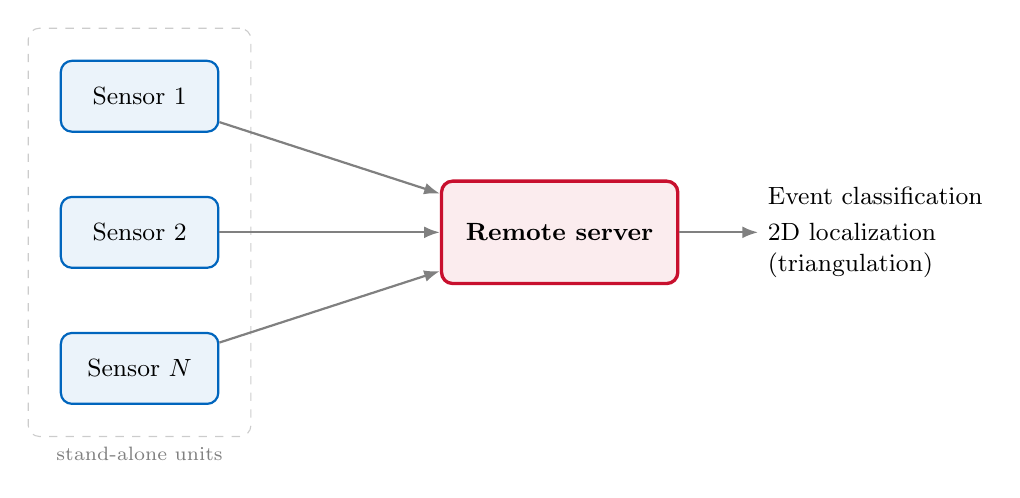
\begin{tikzpicture}[
      node distance=8mm,
      sensor/.style={draw=ctublue,thick,rounded corners,fill=ctublue!8,
                     minimum width=20mm,minimum height=9mm,font=\small},
      server/.style={draw=accent,very thick,rounded corners,fill=accent!8,
                     minimum width=30mm,minimum height=13mm,font=\small\bfseries},
      link/.style={-{Latex[length=2mm]},draw=gray,thick}
    ]
    \node[sensor] (s1) {Sensor 1};
    \node[sensor,below=of s1] (s2) {Sensor 2};
    \node[sensor,below=of s2] (s3) {Sensor $N$};
    \node[server,right=28mm of s2] (srv) {Remote server};

    \draw[link] (s1) -- (srv);
    \draw[link] (s2) -- (srv);
    \draw[link] (s3) -- (srv);

    \node[right=10mm of srv,align=left,font=\small] (out) {
      Event classification\\[2pt]
      2D localization\\(triangulation)};
    \draw[link] (srv) -- (out);

    \begin{scope}[on background layer]
      \node[fit=(s1)(s3),draw=gray!40,dashed,rounded corners,
            inner sep=4mm,label={[font=\scriptsize\color{gray}]below:stand-alone units}] {};
    \end{scope}
  \end{tikzpicture}
  \end{center}
  \vfill
  \begin{itemize}\small
    \item Each sensor continuously monitors its surroundings and transmits detected
          signals to the server for advanced processing.
    \item Multiple units give broader coverage and adaptability to environments.
    \item Tested with various firearm calibers and ammunition.
  \end{itemize}
  \note{%
    \textbf{[3:00--4:00]}\par\medskip
    Here is the system. // Each sensor is a stand-alone unit. It listens
    continuously, and when it detects something impulsive, it sends that signal to
    a remote server. //\par\medskip
    The server does two things. It classifies the event --- is this a gunshot, and
    what kind. And it determines where the event happened, in two dimensions.
    //\par\medskip
    Why multiple units? Two reasons. Coverage --- one unit hears one neighbourhood.
    And localization --- you need at least two bearings to get a position, and I will
    show you that on the next slide. //\par\medskip
    The system has been tested with several firearm calibers and several types of
    ammunition. //
  }
\end{frame}

\begin{frame}{Locating the source}
  \begin{columns}[T,onlytextwidth]
    \begin{column}{0.56\textwidth}
      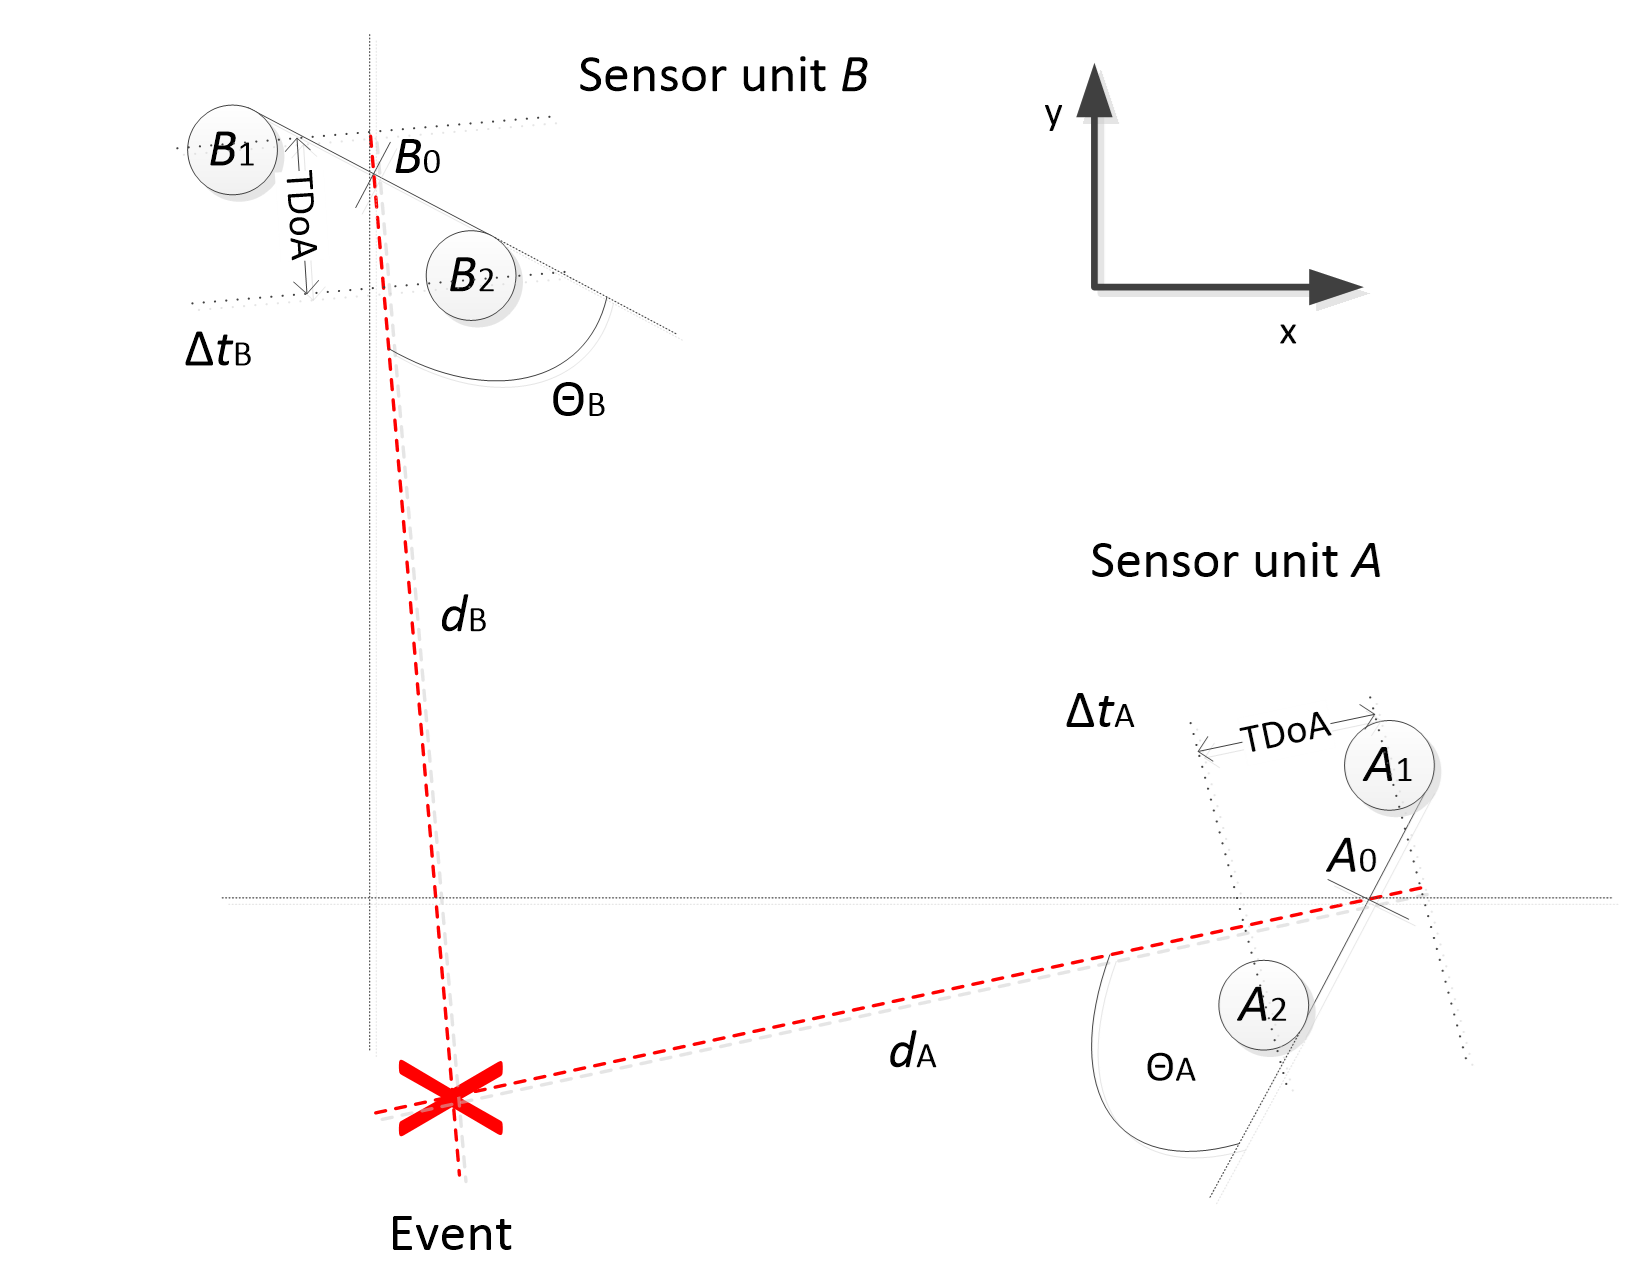
\includegraphics[width=0.96\textwidth]{figs/tdoa.png}
    \end{column}
    \begin{column}{0.42\textwidth}
      \vspace{4mm}
      \[ \Theta = \arcsin\!\left(\frac{c\,\Delta n}{d\,f_s}\right) \]
      \vspace{1mm}
      \begin{itemize}\small
        \item Two MEMS microphones per unit ($d = 0.186$\,m, $f_s = 44.1$\,kHz)
              give one \textbf{bearing} $\Theta$.
        \pause
        \item Two units, two bearings --- they \textbf{intersect} at the event.
        \item Measured: cross-correlation with parabolic interpolation,
              \gtcc{MAE $0.77^\circ$} over 70 events ($-45^\circ$ to $+60^\circ$).
      \end{itemize}
    \end{column}
  \end{columns}
  \note<2>{%
    \textbf{[4:00--5:00]}\par\medskip
    So how do we actually find the shooter? //\par\medskip
    Each sensor unit carries two MEMS microphones, eighteen point six centimetres
    apart. // The sound reaches one microphone before the other. That delay is
    tiny --- at most twenty-four samples at forty-four kilohertz --- but it is enough.
    //\par\medskip
    From it we compute the bearing to the source, theta: the speed of sound times
    the delay in samples, divided by the microphone spacing times the sampling
    frequency. //\par\medskip
    \textbf{[CLICK]}\par\medskip
    One unit gives you a direction. Two units give you two directions, and where
    they cross is the position. //\par\medskip
    We measured how good that bearing is. Using cross-correlation with parabolic
    interpolation, over seventy recorded events, the mean absolute error is zero
    point seven seven degrees. //
  }
\end{frame}

% ===========================================================================
\section{Features}

\begin{frame}{Feature extraction --- cepstral coefficients}
  \begin{center}
  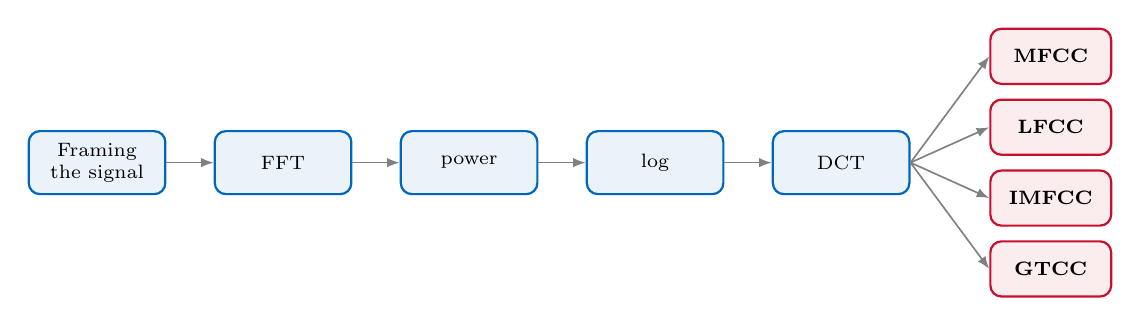
\begin{tikzpicture}[
      node distance=6mm,
      blk/.style={draw=ctublue,thick,rounded corners,fill=ctublue!8,
                  minimum height=8mm,font=\scriptsize,text width=15mm,align=center},
      featbox/.style={draw=accent,thick,rounded corners,fill=accent!8,
                  minimum height=7mm,font=\scriptsize\bfseries,text width=13mm,align=center},
      ar/.style={-{Latex[length=1.6mm]},draw=gray,semithick}
    ]
    \node[blk] (fr) {Framing the signal};
    \node[blk,right=of fr] (fft) {FFT};
    \node[blk,right=of fft] (pw) {power};
    \node[blk,right=of pw] (lg) {log};
    \node[blk,right=of lg] (dct) {DCT};

    \draw[ar] (fr) -- (fft);
    \draw[ar] (fft) -- (pw);
    \draw[ar] (pw) -- (lg);
    \draw[ar] (lg) -- (dct);

    \node[featbox,right=10mm of dct,yshift=13.5mm] (o1) {MFCC};
    \node[featbox,right=10mm of dct,yshift=4.5mm]  (o2) {LFCC};
    \node[featbox,right=10mm of dct,yshift=-4.5mm] (o3) {IMFCC};
    \node[featbox,right=10mm of dct,yshift=-13.5mm](o4) {GTCC};
    \foreach \o in {o1,o2,o3,o4} \draw[ar] (dct.east) -- (\o.west);
  \end{tikzpicture}
  \end{center}
  \vspace{2mm}
  {\scriptsize Block diagram of the feature extraction algorithms (Fig.~1 in the abstract);
   each branch applies its own filter bank before the DCT.}
  \vfill
  \begin{itemize}\small
    \item MFCC was developed for other acoustic applications but works for gunshot
          recognition --- validated at military shooting ranges.
    \item LFCC and IMFCC offer alternative filtering approaches.
    \item GFCC and GTCC derive from human auditory response models; \textbf{GTCC is
          more noise-resistant than MFCC}.
  \end{itemize}
  \note{%
    \textbf{[5:00--6:15]}\par\medskip
    Now the classification. // The feature extractor is based on cepstral
    coefficients. The chain is the same for all of them: cut the signal into
    frames, take the FFT, take the power, take the logarithm, and finish with a
    discrete cosine transform. //\par\medskip
    What differs is one step that is not drawn here --- the filter bank that sits
    before the DCT. //\par\medskip
    Mel-frequency coefficients, MFCC, were developed for speech, but they work for
    gunshots; that has been validated at military shooting ranges. // LFCC uses
    linear spacing, IMFCC an inverted mel scale. // And GTCC uses a gammatone filter
    bank, which models the response of the human ear. It is known to be more
    noise-resistant than MFCC. //\par\medskip
    We tested all four, at three frame lengths --- fifteen, thirty and fifty
    milliseconds --- with two classifiers: a neural network and a support vector
    machine. //
  }
\end{frame}

% ===========================================================================
\section{Results}

\begin{frame}{Classification results --- 9\,mm class}
  \centering
  \footnotesize
  \begin{tabular}{ll rr rr rr}
    \toprule
    & & \multicolumn{2}{c}{ACC (\%)} & \multicolumn{2}{c}{RLC (\%)} & \multicolumn{2}{c}{MCC (--)}\\
    \cmidrule(lr){3-4}\cmidrule(lr){5-6}\cmidrule(lr){7-8}
    Frame & Extractor & SVM & NN & SVM & NN & SVM & NN\\
    \midrule
    15\,ms & MFCC  & 83.90 & 85.59 & 80.65 & 67.74 & 0.62 & 0.62\\
           & LFCC  & 83.90 & 83.90 & 80.65 & 64.52 & 0.62 & 0.57\\
           & IMFCC & 85.59 & 90.68 & 83.87 & 87.10 & 0.66 & 0.77\\
           & \gtcc{GTCC} & \gtcc{93.22} & \gtcc{97.46} & \gtcc{87.10} & \gtcc{93.55} & \gtcc{0.82} & \gtcc{0.93}\\
    \midrule
    30\,ms & MFCC  & 84.75 & 87.29 & 67.74 & 87.10 & 0.60 & 0.70\\
           & LFCC  & 87.29 & 83.90 & 70.97 & 70.97 & 0.66 & 0.59\\
           & IMFCC & 85.59 & 92.37 & 67.74 & 80.65 & 0.62 & 0.80\\
           & \gtcc{GTCC} & \gtcc{97.46} & \gtcc{98.31} & \gtcc{90.32} & \gtcc{93.55} & \gtcc{0.93} & \gtcc{0.96}\\
    \midrule
    50\,ms & MFCC  & 84.75 & 93.22 & 74.19 & 90.32 & 0.61 & 0.83\\
           & LFCC  & 88.98 & 86.44 & 77.42 & 77.42 & 0.71 & 0.66\\
           & IMFCC & 89.83 & 90.68 & 74.19 & 80.65 & 0.73 & 0.76\\
           & \gtcc{GTCC} & \gtcc{97.46} & \gtcc{99.15} & \gtcc{90.32} & \gtcc{96.77} & \gtcc{0.93} & \gtcc{0.98}\\
    \bottomrule
  \end{tabular}
  \par\vspace{2mm}
  {\scriptsize Table~I in the abstract --- example of classification results for a 9\,mm class.
   Test partition: 118 events, 31 of them 9\,mm.}
  \note{%
    \textbf{[6:15--7:45]}\par\medskip
    This is the result table for the nine-millimetre class. Let me walk you through
    it. //\par\medskip
    The rows are grouped by frame length --- fifteen, thirty, fifty milliseconds ---
    and inside each group you see the four extractors. // The columns are three
    metrics, each for both classifiers: accuracy, recall, and the Matthews
    correlation coefficient. //\par\medskip
    Now look only at the red rows. That is GTCC. // At every single frame length,
    and for both classifiers, GTCC is the best row in its block. //\par\medskip
    The best cell in the table is GTCC with the neural network at fifty
    milliseconds: ninety-nine point one five percent accuracy, ninety-six point
    seven seven percent recall, and a Matthews coefficient of zero point nine
    eight. //\par\medskip
    To put those numbers in context --- the test set has one hundred and eighteen
    events, thirty-one of them nine-millimetre. So that accuracy is one hundred and
    seventeen correct out of one hundred and eighteen, and that recall is thirty
    shots out of thirty-one. //
  }
\end{frame}

\begin{frame}{What the numbers say}
  \begin{itemize}
    \item \textbf{MFCC, LFCC and IMFCC yield similar results.}
    \item \gtcc{GTCC consistently performs better} across every frame length and both
          classifiers.
    \item \textbf{NN outperforms SVM} --- better at modelling complex patterns.
          The gap widens with longer frames.
    \item \textbf{Longer frames improve accuracy}, but start to capture environmental
          reflections, which can pull focus away from the gunshot itself.
  \end{itemize}
  \vfill
  \begin{block}{Best configuration in the table}
    GTCC + NN at 50\,ms --- 99.15\,\% ACC, 96.77\,\% RLC, MCC 0.98.
  \end{block}
  \note{%
    \textbf{[7:45--8:45]}\par\medskip
    Three things come out of this. //\par\medskip
    First, MFCC, LFCC and IMFCC behave almost identically. Changing the shape of a
    mel-type filter bank does not buy you much. //\par\medskip
    Second, GTCC is consistently better --- every frame length, both classifiers. The
    gammatone filter bank resolves the low frequencies more finely, and that is
    exactly where the energy of a muzzle blast sits. //\par\medskip
    Third, the neural network beats the support vector machine, and the gap grows
    with longer frames. //\par\medskip
    And about those longer frames --- they do improve accuracy, but remember the
    reflections I showed you at the beginning. A fifty-millisecond frame starts to
    include the acoustics of the room instead of the gunshot. So this trend does
    not continue forever. //
  }
\end{frame}

% ===========================================================================
\section{Conclusion}

\begin{frame}{Conclusion}
  \begin{itemize}
    \item A distributed network of stand-alone acoustic sensors with a remote server
          detects, classifies and localizes impulsive sounds in 2D.
    \item Cepstral coefficients are an effective feature extractor for gunshot
          classification with both NN and SVM.
    \item GTCC beats Mel-frequency based coefficients; NN achieves slightly better
          classification success, especially with longer frames.
    \item Validated with various firearm calibers and ammunition.
  \end{itemize}
  \vfill
  \centering
  \vspace{3mm}
  {\large Thank you --- questions?}\\[2mm]
  {\small\color{gray} svatoja1@fel.cvut.cz \quad maxamart@fel.cvut.cz}
  \note{%
    \textbf{[8:45--9:30]}\par\medskip
    To summarise. //\par\medskip
    We built a distributed network of stand-alone acoustic sensors with a remote
    server, which detects, classifies and localizes impulsive sounds in two
    dimensions. //\par\medskip
    Cepstral coefficients work well as a feature extractor for gunshot
    classification, with both classifiers. // Gammatone-based coefficients beat the
    mel-frequency family, and the neural network is slightly better than the SVM,
    especially at longer frames. //\par\medskip
    And all of this was validated with real firearms, several calibers and several
    types of ammunition. //\par\medskip
    Thank you. I am happy to take questions. //
  }
\end{frame}

% ===========================================================================
\appendix

\begin{frame}{Backup --- experimental setup and dataset}
  \begin{columns}[T,onlytextwidth]
    \begin{column}{0.46\textwidth}
      \small
      \begin{itemize}
        \item Military shooting range, fixed sensor position, clear line of sight to
              every firing position.
        \item Four weapons: 9\,mm, 5.56 NATO SD, 7.62\,mm Tokarev, .22 --- each with a
              single ammunition type.
        \item Plus a false-alarm class with gunshot-like impulsive patterns.
        \item 26 features per extractor; $\approx$75\,/\,25 train--test split.
        \item NN: MATLAB Neural Fitting, Levenberg--Marquardt, 370 iterations.
      \end{itemize}
    \end{column}
    \begin{column}{0.5\textwidth}
      \centering\footnotesize
      \begin{tabular}{llrr}
        \toprule
        \multicolumn{2}{l}{Class} & Train & Test\\
        \midrule
        0 & False alarms      &  86 &  21\\
        1 & \gtcc{9\,mm}      &  \gtcc{70} &  \gtcc{31}\\
        2 & 5.56 NATO SD      & 100 &  31\\
        3 & 7.62\,mm Tokarev  &  55 &  17\\
        4 & .22               &  60 &  18\\
        \midrule
        \multicolumn{2}{l}{Total} & \textbf{371} & \textbf{118}\\
        \bottomrule
      \end{tabular}
      \par\vspace{2mm}
      {\scriptsize Svatoš \& Holub, \emph{Meas. Sci. Technol.} \textbf{35} (2024) 076122,
       Table~2.}
    \end{column}
  \end{columns}
\end{frame}

\begin{frame}{Backup --- bearing estimation methods}
  \centering
  \footnotesize
  \begin{tabular}{lrrr}
    \toprule
    Method & MAE & Median & Max\\
    \midrule
    Cross-correlation                      & $0.84^\circ$ & $0.41^\circ$ & $7.61^\circ$\\
    \gtcc{Cross-correlation + parabolic interp.} & \gtcc{$0.77^\circ$} & \gtcc{$0.56^\circ$} & \gtcc{$6.67^\circ$}\\
    Phase-based delay estimation (PBDE)    & $3.24^\circ$ & $1.80^\circ$ & $29.0^\circ$\\
    PBDE + linear regression               & $3.91^\circ$ & $3.55^\circ$ & $12.15^\circ$\\
    \bottomrule
  \end{tabular}
  \vspace{2mm}

  {\scriptsize 70 events, 9 reference angles from $-45^\circ$ to $+60^\circ$,
   $d = 0.186$\,m, $f_s = 44.1$\,kHz.}
  \vfill
  \begin{columns}[T,onlytextwidth]
    \begin{column}{0.48\textwidth}
      \small\textbf{PBDE algorithm}
      \begin{enumerate}\small
        \item FFT of both channels
        \item select the relevant frequency bins
        \item phase angle $\varphi = \arg(S_1 S_2^{*})$
        \item delay from the phase slope
      \end{enumerate}
    \end{column}
    \begin{column}{0.48\textwidth}
      \small\textbf{How many units for 2D?}
      \begin{itemize}\small
        \item ToA, 1 mic per unit --- 3 units
        \item TDoA, 1 mic per unit --- 4 units
        \item \textbf{TDoA, 2 mics per unit --- 2 units}
      \end{itemize}
    \end{column}
  \end{columns}
\end{frame}

\begin{frame}{Backup --- other cepstral coefficients}
  \begin{itemize}
    \item \textbf{LPCC} (Linear Prediction Cepstral Coefficients) and \textbf{PLPC}
          (Perceptual Linear Prediction Coefficients) --- noise elimination, speech
          recognition.
    \item \textbf{GFCC} (Greenwood Function Cepstral Coefficients) --- derived from
          human auditory response models, used for classifying animal sounds.
    \item \textbf{GTCC} (Gammatone-Frequency Cepstral Coefficients) --- same family,
          greater resistance to noise than MFCC.
  \end{itemize}
\end{frame}

\begin{frame}{Backup --- metrics}
  \begin{description}
    \item[ACC] Accuracy --- share of correctly classified events.
    \item[RLC] Recall, also known as \emph{sensitivity} --- share of actual gunshots
      of the class that were detected.
    \item[MCC] Matthews Correlation Coefficient --- balanced measure robust to class
      imbalance; $+1$ perfect, $0$ random.
  \end{description}
  \vfill
  {\small\color{gray} Definitions as used in the source study: Svatoš \& Holub,
   \emph{Meas. Sci. Technol.} \textbf{35} (2024) 076122, eqs.~(1)--(3).}
\end{frame}

\end{document}
